% Chapter Template

\chapter{The Receiver} % Main chapter title

\label{Chapter5}

\section{Introduction}

The receiver for the sound-based move tracking protocol is in charge of
decoding a sequence of face turns from the transmitted audio.

To do this, the receiver must go through the following steps:

\begin{enumerate}
    
    \item Record the transmitted audio.q
    
    \item Measure the audible frequencies at each time step.
    
    \item Convert each time step's audible frequencies to the cube's
    state at that moment.
    
    \item Decode the applied face turns from the sequence of cube
    states.

\end{enumerate}

This chapter will describe the development of a software algorithm in
Python that can serve as a receiver for this sound-based move tracking
protocol. This development began with the creation of synthetic audio
recordings representing the tones that would be emitted by a Rubik's
Cube equipped with an ideal transmitter (Section
\ref{sec:synthetic-audio-generation}) followed by the implementation of
an algorithm capable of decoding that ideal synthetic audio (Section
\ref{sec:decoding-synthetic-audio}). The algorithm was then made more
robust by adding realistic noise to the synthetic audio to better
simulate a real speedcubing environment (Section
\ref{sec:adding-realistic-noise}) followed by enhancing the previously
designed algorithm to continue to decode the applied move sequence in
the midst of the added noise (Section:
\ref{sec:decoding-realistic-noise}). \footnote{The contents of this
chapter have been specially written so that the reader can copy them
into a Jupyter Notebook running a Python 3.9 kernel and see the same
results for himself/herself.}


\section{Creating Synthetic Audio}
\label{sec:synthetic-audio-generation}

The first step of designing this receiver is to synthesize an audio
signal representative of the output of the ideal transmitter.

This audio synthesis starts with encoding the frequency corresponding
to each centerpiece state (Section
\ref{subsec:represent-audio-protocol}), then involves creating a
virtual Rubik's Cube (Section \ref{subsec:represent-rubiks-cube}), and
finally culminates in generating the audio signal from the virtual
Rubik's Cube's state (Section \ref{subsec:generate-audible-algorithm}).

\newpage
\subsection{Representing the Audio Protocol}
\label{subsec:represent-audio-protocol}

For the synthetic audio generator to produce a realistic signal, it
needs to know which frequencies to transmit for each centerpiece state.
This is easily accomplished by creating a dictionary to map each
possible state of each face to its corresponding frequency.

For this design, the frequency assignments from Table
\ref{table:centerpiece-frequencies} are converted to the dictionary
shown in Figure \ref{fig:code-freq-mapping-dict} with two small
changes. First, by assuming no cube rotations, the face color (e.g.
"White") can be converted to a layer name (e.g. "U") which simplifies
the code for both encoding and decoding a move sequence from audio.
Second, the 0$^\circ$, 90$^\circ$, 180$^\circ$, and 270$^\circ$
alignments from Figure \ref{fig:rotation-alignment} are divided by 90
to be represented by the simple sequence of consecutive integers 0, 1,
2, and 3 that are easier to manipulate in code.

With this dictionary in place, the frequency to transmit for any
particular centerpiece's current rotation can be determined by looking
up the centerpiece and its rotation in the dictionary as shown in
Figure \ref{fig:code-frequency-of}.

\begin{figure}[h]
\caption{Centerpiece State to Frequency Mapping}
\begin{subfigure}{\textwidth}
\caption{Frequency mapping dictionary}
\label{fig:code-freq-mapping-dict}
\begin{lstlisting}[language=Python]
FREQUENCY_MAPPINGS = {
    "U": {
        0: 800, 1: 900, 2: 1000, 3: 1100
    },
    "D": {
        0: 1300, 1: 1400, 2: 1500, 3: 1600
    },
    "R": {
        0: 1800, 1: 1900, 2: 2000, 3: 2100
    },
    "L": {
        0: 2300, 1: 2400, 2: 2500, 3: 2600
    },
    "F": {
        0: 2800, 1: 2900, 2: 3000, 3: 3100
    },
    "B": {
        0: 3300, 1: 3400, 2: 3500, 3: 3600
    }
}
\end{lstlisting}
\end{subfigure}\\
\begin{subfigure}{\textwidth}
\caption{Frequency lookup function}
\label{fig:code-frequency-of}
\begin{lstlisting}[language=Python, firstnumber=last]
def frequency_of(centerpiece: str, rotation: int) -> float:
    return FREQUENCY_MAPPINGS[centerpiece][rotation]
\end{lstlisting}
\end{subfigure}
\end{figure}


\newpage
\subsection{Representing the Rubik's Cube}
\label{subsec:represent-rubiks-cube}

While there are many implementations of a digital Rubik's Cube that can
track every cubie and render an interactive 3D cube, all that's needed
for the synthetic audio generator is a representation of a Rubik's Cube
on which individual face turns can be virtually applied and the

resulting centerpiece state can be read out. To do this, a
\code{RubiksCube} object is created that encapsulates a dictionary
containing the same keys for each face as the
\code{FREQUENCY\_MAPPINGS} dictionary in Figure
\ref{fig:code-freq-mapping-dict} above, each associated with a single
integer representing the current rotational state of that face. A
method called \code{apply\_move} is also defined with a parameter for a
valid move like \code{U} or \code{U'} that will update the
\code{RubiksCube}'s state to reflect the rotation.

\begin{figure}[h]
\caption{A simple abstraction of a Rubik's Cube}
\label{fig:rubiks-cube-code}
\begin{lstlisting}[language=Python]
class RubiksCube:
    
    CLOCKWISE = 1           # aka a 90 degree turn
    COUNTERCLOCKWISE = 3    # aka a 270 degree turn which achieves the
                            # same resulting state as a -90 degree turn

    def __init__(self):
        self.state = { "U": 0, "D": 0, "R": 0, "L": 0, "F": 0, "B": 0 }
    
    def apply_move(self, move: str):
        # Extract the face and direction from the `move` string.
        face = move[0]
        if len(move) == 1:                             # e.g. U
            direction = RubiksCube.CLOCKWISE
        else:                                          # e.g. U'
            direction = RubiksCube.COUNTERCLOCKWISE
        
        # Update the state to apply the move.
            # NOTE: The `mod 4` exists to wrap back around to 0
            # after a full 360 degrees of rotation.
        self.state[face] = (self.state[face] + direction) % 4
\end{lstlisting}
\end{figure}

\subsection{Creating Synthetic Audio for an Arbitrary Algorithm}
\label{subsec:generate-audible-algorithm}

Now the synthetic audio can be generated for any valid algorithm. This
is done using the \code{tones} library created by Erik Nyquist.
\cite{pip-tones}

First, a separate audio track is created to simulate the output of each
speaker embedded into each centerpiece on the cube (Figure
\ref{fig:code-create-mixer}).

Second, a new function is written to add the tones corresponding to the
virtual cube's current state to the audio mixer using the
\code{frequency\_of} function from Figure \ref{fig:code-frequency-of}
(Figure \ref{fig:code-render-cube-state}). This function includes a
\code{tps} parameter that controls the duration of the added tones so
that they change to the next tone at the same speed as the turns on a
speedcube being solved at that number of turns per second.

Then, those two functions are tied together by iterating through each
move in a Rubik's Cube \code{alg}orithm and saving the audio of the
resulting state changes into a .wav file at a given file path (Figure
\ref{fig:code-render-audible-alg}). Additionally, the \code{tps}
parameter is propagated to this function to enable generating audio for
an algorithm at different turn speeds.

\begin{figure}[h]
\caption{Generating audio for any Rubik's Cube algorithm}
\label{fig:code-generate-alg-audio}
\begin{subfigure}{\textwidth}
\caption{Function to create an audio mixer for a virtual Rubik's Cube}
\label{fig:code-create-mixer}
\begin{lstlisting}[language=Python]
from tones.mixer import Mixer  # https://pypi.org/project/tones/
from tones import SINE_WAVE

def _create_mixer(rubiks_cube: RubiksCube) -> Mixer:
    mixer: Mixer = Mixer(sample_rate=44100, amplitude=1)
    # Add a separate audio track for each centerpiece.
    for face, _ in rubiks_cube.state.items():
        mixer.create_track(face, SINE_WAVE, attack=0, decay=0)
    return mixer
\end{lstlisting}
\vspace*{2mm}
\end{subfigure}\\
\begin{subfigure}{\textwidth}
\caption{Function to update an audio mixer with a virtual Rubik's Cube's state}
\label{fig:code-render-cube-state}
\begin{lstlisting}[language=Python, firstnumber=last]
def _render_cube_state(mixer: Mixer, rubiks_cube: RubiksCube, tps: float):
    for face, rotation in rubiks_cube.state.items():
        mixer.add_tone(face, frequency_of(face, rotation), duration=1 / tps)
\end{lstlisting}
\vspace*{2mm}
\end{subfigure}\\
\begin{subfigure}{\textwidth}
\caption{Function to create a .wav file of any Rubik's Cube algorithm}
\label{fig:code-render-audible-alg}
\begin{lstlisting}[language=Python, firstnumber=last]
def render_audible_alg(alg: str, wav_path: str=None, tps: float=4):
    # Create the virtual Rubik's Cube.
    rubiks_cube: RubiksCube = RubiksCube()
    # Create the audio mixer used to create the synthesized audio.
    mixer = _create_mixer(rubiks_cube)
    # Add the initial cube state to the mixer.
    _render_cube_state(mixer, rubiks_cube, tps)
    # Iterate over the alg, updating the mixer after each move.
    moves = alg.split(" ")
    for move in moves:
        rubiks_cube.apply_move(move)
        _render_cube_state(mixer, rubiks_cube, tps)
    # Save the final audio to a .wav file.
    mixer.write_wav(wav_path if wav_path else f"{alg}.wav")
\end{lstlisting}
\end{subfigure}
\end{figure}

With these functions in place, synthetic audio can be easily created
for any valid Rubik's Cube algorithm. For example, generating synthetic
audio that sweeps through every possible centerpiece state can be done
with the two lines of code in Figure \ref{fig:example-alg-audio}.

\begin{figure}[h]
\caption{Example Audio Generation for a Rubik's Cube Algorithm}
\label{fig:example-alg-audio}
\begin{lstlisting}[language=Python]
demo_alg = "U U U U D D D D R R R R L L L L F F F F B B B B"
render_audible_alg(demo_alg, "demo_all_states.wav")
\end{lstlisting}
\end{figure}


\section{Decoding the Synthetic Audio}
\label{sec:decoding-synthetic-audio}

With synthetic audio now available for any valid Rubik's Cube
algorithm, the next step is to create an initial software algorithm
that can decode that audio back into the original move sequence.

Accomplishing this will require computing the synthetic audio's
spectrogram (Section \ref{subsec:compute-spectrogram}), followed by
extracting the dominant frequencies present at each time step (Section
\ref{subsec:extract-dominant-freqs}), and converting those dominant
frequencies into the corresponding Rubik's Cube centerpiece states
(Section \ref{subsec:translating-freqs-to-state}), all before finally
recovering the originally applied move sequence (Section
\ref{subsec:extract-moves}).

\subsection{Computing the Spectrogram}
\label{subsec:compute-spectrogram}

The first step in decoding the synthetic audio is determining its
component frequencies at any specific moment in time. These component
frequencies can be easily visualized using a spectrogram, like the one
in Figure \ref{fig:spectrogram} of the synthetic audio created in
Section \ref{subsec:generate-audible-algorithm}. \footnote{The source
code for Figure \ref{fig:spectrogram} is available in Appendix
\ref{sec:code-spectrogram}.}

\begin{figure}[h]
    \centering
    \caption{Spectrogram of the synthetic audio created in Section \ref{subsec:generate-audible-algorithm}}
    \label{fig:spectrogram}
    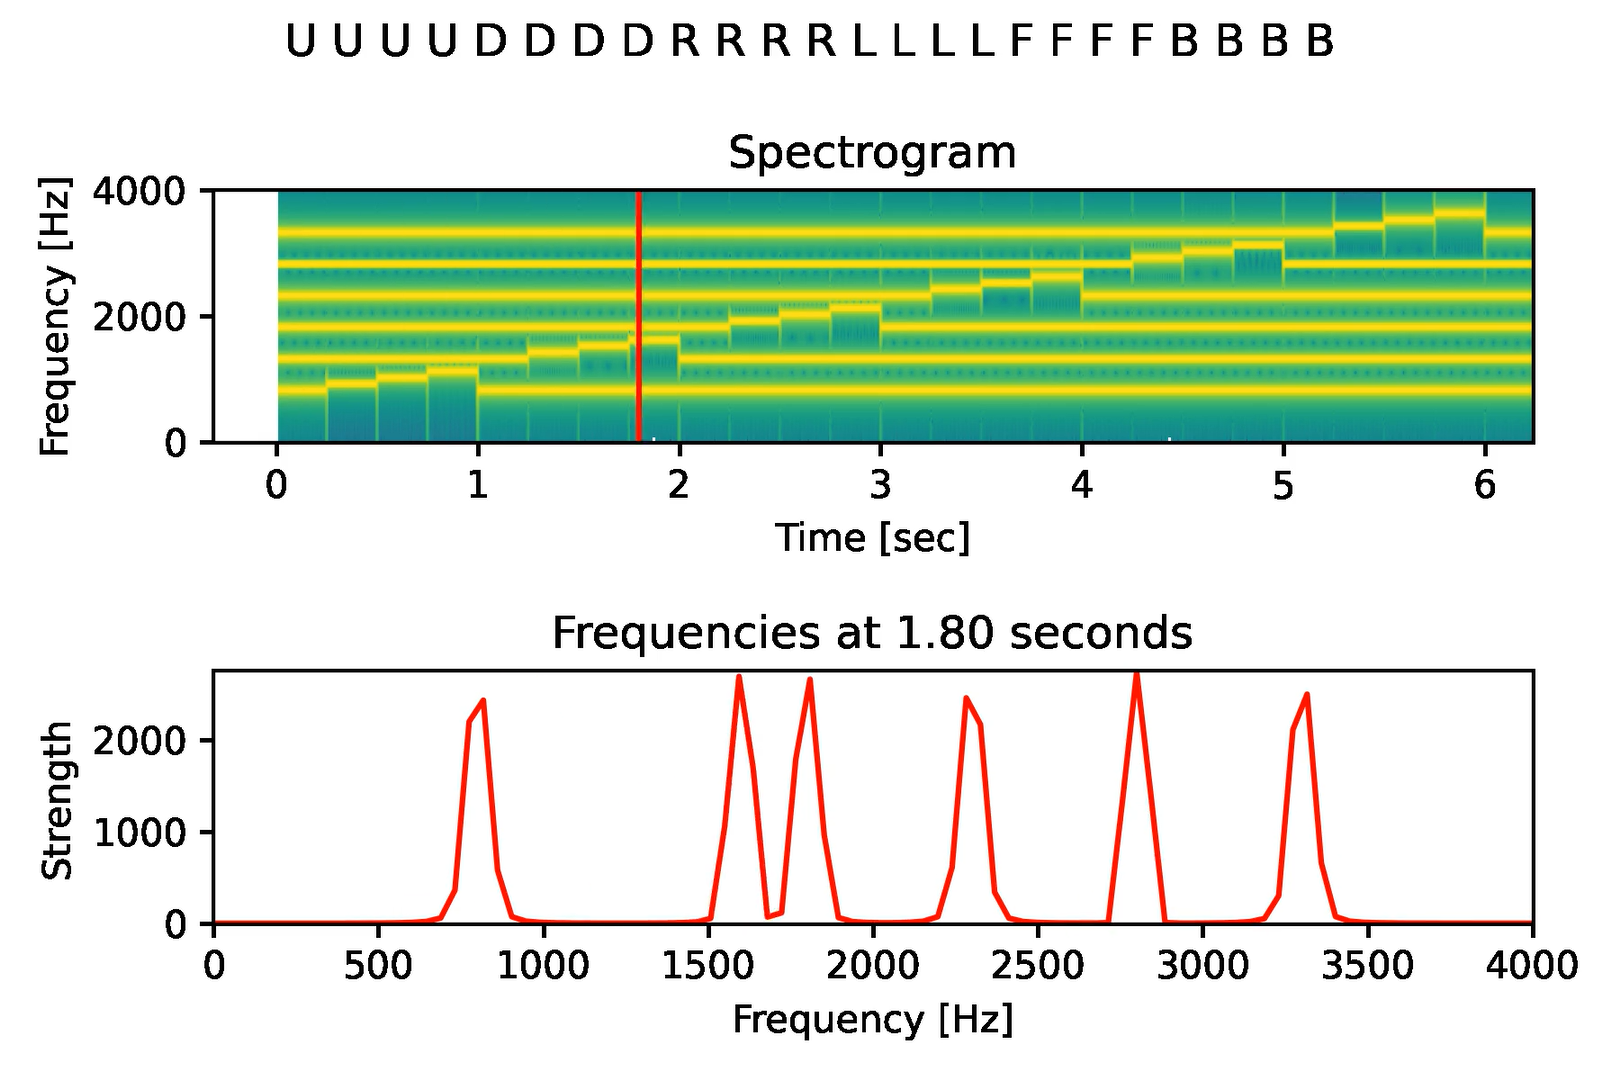
\includegraphics[width=0.8\textwidth]{Figures/5 Algorithm Design/component_frequencies.png}
\end{figure}

This spectrogram has the same pieces as the ones described in Section
\ref{subsubsec:how-to-read-a-spectrogram} with a few minor changes.
First the order of the graphs has been reversed, so the top graph shows
the actual spectrogram and the bottom graph shows the strength of the
component frequencies at the specific point in time indicated by the
vertical red line on the top graph. Additionally, the spectrogram has
been rotated 90$^\circ$ so time is now on the x-axis and the component
frequencies are shown on the y-axis. Finally, the color scheme is
slightly different, with the presence of a strong component frequency
indicated by a bright yellow color instead of bright purple or pink.

\subsubsection{The Brief Overview of the Math behind the Spectrogram}

However, while Matplotlib's \code{specgram} plot \cite{matplotlib} made
it easy to create Figure \ref{fig:spectrogram}, it didn't return the
underlying data of the spectrogram required to decode the exact values
and strengths of the component frequencies at each point in time. To
compute that data directly, it is helpful to understand the basics of
the math behind the spectrogram. Dr. Steve Brunton from the University
of Washington created an excellent video series on this topic
\cite{fourier-analysis}, of which the following few paragraphs are a
short summary.

The foundational mathematical concept behind the spectrogram is the
Fourier Transform, which is a technique for approximating any
continuous function using only sine and cosine functions. In the case
of an analog audio signal -which is inherently a composite of many sine
functions (one for each component frequency)- applying a Fourier
Transform would return data for a graph of all the frequencies present
at any point in the entire signal and their overall strength throughout
it.

But digital audio signals like .wav files are a series of discrete
values, not continuous functions, which means the Fourier Transform
cannot directly operate on them. Fortunately, there exists a variant of
the Fourier Transform called the Discrete Fourier Transform which can
operate on a list of discrete data points by assuming they sample a
continuous function and then computing the Fourier Transform of that
function.

However, when applied to a digital audio signal, the Discrete Fourier
Transform still only computes which frequencies were present at
\emph{any} time during the duration of the signal, but not \emph{when}
they occurred. That data comes from another layer of computation called
the Gabor Transform (i.e. the Short-Time Fourier Transform) which
computes a Discrete Fourier Transform over a sliding window of the
input samples to approximate the changes in the strength of each
component frequency over time.

This knowledge, combined with the \code{numpy} \cite{numpy} and
\code{scipy} \cite{scipy} libraries which can calculate these
transforms, enables the creation of a function (Figure
\ref{fig:code-compute-spectrogram}) to compute the spectrogram for the
audio stored in a given .wav file. The return values \code{freq} and
\code{time} are, respectively, lists of the .wav file's component
frequencies and time steps, while \code{spectrogram} is a 2D array of
the strengths of each component frequency at each time step. They are
related by common indices, such that the strength of the frequency
\code{freq[f\_idx]} at the time \code{time[t\_idx]} is found in
\code{spectrogram[t\_idx][f\_idx]}.

\begin{figure}[h]
\caption{Function to compute the spectrogram of a .wav file}
\label{fig:code-compute-spectrogram}
\begin{lstlisting}[language=Python]
import numpy as np
from scipy import signal
from scipy.io import wavfile

def compute_spectrogram(wav_path: str):
    SAMPLES_PER_WINDOW = 1024  # Balances frequency/time accuracy
    sample_rate, audio_samples = wavfile.read(wav_path)
    freq, time, Zxx = signal.stft(audio_samples, fs=sample_rate,
        nperseg=SAMPLES_PER_WINDOW, noverlap=(SAMPLES_PER_WINDOW // 4) * 3)
    spectrogram = np.abs(Zxx).transpose()
    return freq, time, spectrogram
\end{lstlisting}
\end{figure}

\subsection{Extracting the Dominant Component Frequencies}
\label{subsec:extract-dominant-freqs}

Looking back at the component frequency graph in Figure
\ref{fig:spectrogram} it is clear that it has six distinct peaks: these
are the transmitted frequencies representing the current state of the
virtual Rubik's Cube's six centerpieces at that specific instant of
time.

The exact frequencies of these peaks can be extracted by filtering out
all frequencies whose strength is not above a specific threshold. In
this case, a simple threshold of 85\% of the maximum strength of any
component frequency (see the green line in Figure
\ref{fig:spectrogram-with-naive-threshold}\footnote{The source code for
Figure \ref{fig:spectrogram-with-naive-threshold} is available in
Appendix \ref{sec:code-spectrogram-with-naive-threshold}.}) isolates
the six dominant component frequencies.

\begin{figure}[h]
    \centering
    \caption{Spectrogram from Figure \ref{fig:spectrogram} with a threshold at 85\% of the maximum strength of the component frequencies. }
    \label{fig:spectrogram-with-naive-threshold}
    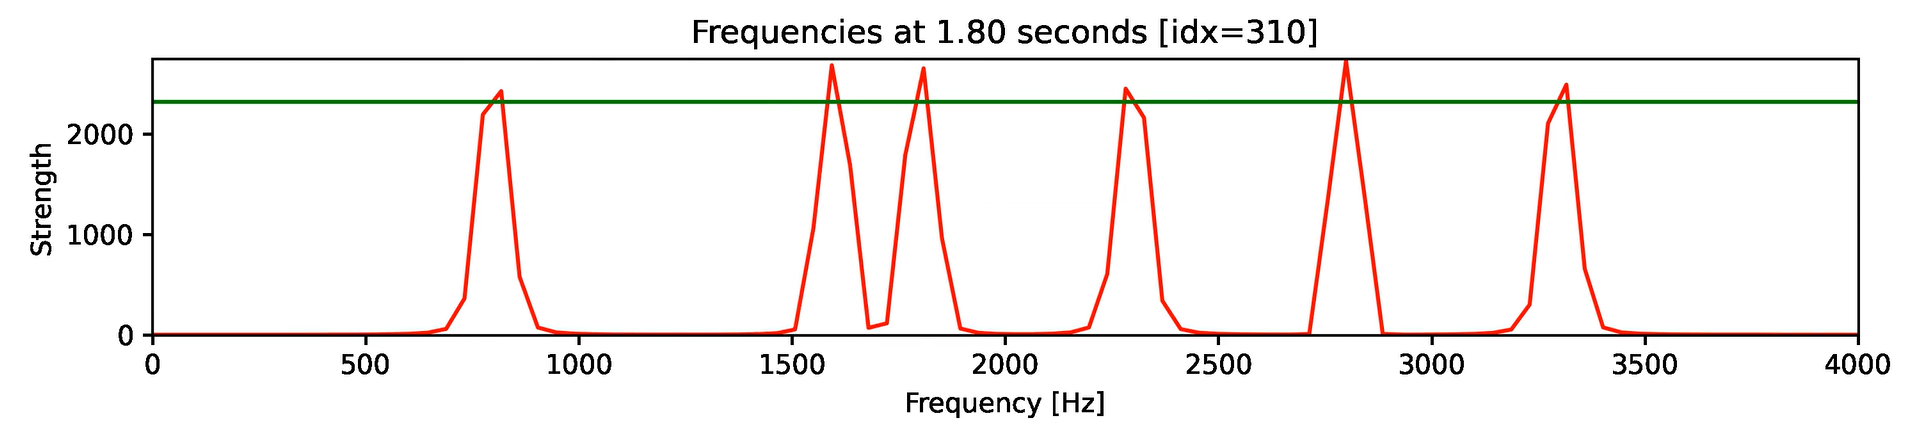
\includegraphics[width=0.8\textwidth]{Figures/5 Algorithm Design/threshold.png}
\end{figure}

Using the actual spectrogram data, the exact values of these peaks can
be computed. First, the threshold computation is broken into its own
function (Figure \ref{fig:code-compute-threshold}). From there, a
second function (Figure \ref{fig:code-extract-important-freqs}) can
iterate through all the component frequencies of the computed
spectrogram data at a specific time index to compile and return a list
of the frequencies whose strength exceeds the threshold at that time
step.

\begin{figure}[h]
\caption{Extracting dominant frequencies from one time step of audio}
\label{fig:code-extract-dominant-freqs}

\begin{subfigure}{\textwidth}
\caption{Function to calculate a simple threshold to isolate the most dominant frequencies}
\label{fig:code-compute-threshold}
\begin{lstlisting}[language=Python]
def compute_threshold(values: list):
    return max(values) * 0.85
\end{lstlisting}
\vspace*{2mm}
\end{subfigure}\\

\begin{subfigure}{\textwidth}
\caption{Function to extract all frequencies stronger than a threshold at a given time step}
\label{fig:code-extract-important-freqs}
\begin{lstlisting}[language=Python, firstnumber=last]
def extract_important_freqs(freq, time, spectrogram, t_idx):
    # Create a list to store the important frequencies
    important_freqs = []
    # Compute the threshold for this time step
    threshold = compute_threshold(spectrogram[t_idx])
    # Check the strength of each frequency at this time step
    for f_idx in range(len(freq)):
        # If the frequency's strength is above the threshold ...
        if spectrogram[t_idx][f_idx] > threshold:
            # ... save the frequency and its strength for later processing
            important_freqs.append(dict(
                hz=freq[f_idx],
                power=spectrogram[t_idx][f_idx]
            ))
    return important_freqs
\end{lstlisting}
\end{subfigure}\\
\end{figure}

With these functions, finding the actual frequencies of the peaks in
Figure \ref{fig:spectrogram-with-naive-threshold} can be done in just a
few lines of code as shown in Figure
\ref{fig:code-extract-important-freqs-demo}.

\begin{figure}[h]
\caption{Example peak frequency decoding at a specific time step}
\label{fig:code-extract-important-freqs-demo}
\begin{subfigure}{\textwidth}
\begin{lstlisting}[language=Python]
freq, time, spectrogram = compute_spectrogram(demo_wav_path)
important_freqs = extract_important_freqs(
    freq, time, spectrogram, t_idx=310) # 1.80 seconds
print([f"{x["hz"]:.0f}Hz" for x in important_freqs])
\end{lstlisting}
\end{subfigure}\\

\begin{subfigure}{\textwidth}
\begin{lstlisting}[language=Python, numbers=none]
>> ["818Hz", "1593Hz", "1809Hz", "2283Hz", "2799Hz", "3316Hz"]
\end{lstlisting}
\end{subfigure}
\end{figure}

\subsection{Translating Component Frequencies to Centerpiece States}
\label{subsec:translating-freqs-to-state}

With the specific frequencies of each detected peak, the original state
of the Rubik's Cube at that moment in time can be computed by finding
the states whose corresponding frequency is closest to each detected
peak frequency.

This is done by first defining a function that will find the closest
centerpiece state for one peak frequency by iterating through every
centerpiece state in the \code{FREQUENCY\_MAPPINGS} dictionary from
Section \ref{subsec:represent-audio-protocol}, comparing the difference
between the state's frequency and the given peak frequency, and
returning the state with the smallest difference (Figure
\ref{fig:code-closest-state}). This function can then be called for all
the detected peak frequencies to recover the state of the cube at that
time step (Figure \ref{fig:code-get-state-from-freqs}).

\begin{figure}[h]
\caption{Converting peak frequencies to centerpiece states}
\label{fig:code-convert-peak-freqs-to-state}
\begin{subfigure}{\textwidth}
\caption{Function to find the state most similar to the detected frequency}
\label{fig:code-closest-state}
\begin{lstlisting}[language=Python]
def _closest_state(detected_freq):
    # Start with no assumptions regarding the closest state
    closest_state = None
    closest_difference = None
    # Iterate through each possible state to find the closest one
    for face, rotations in FREQUENCY_MAPPINGS.items():
        for rotation, freq in rotations.items():
            difference = abs(detected_freq - freq)
            if closest_difference is None or difference < closest_difference:
                closest_difference = difference
                closest_state = dict(face=face, rotation=rotation)
    return closest_state
\end{lstlisting}
\end{subfigure}\\

\begin{subfigure}{\textwidth}
\caption{Function to determine the cube's state from a set of peak frequencies}
\label{fig:code-get-state-from-freqs} 
\begin{lstlisting}[language=Python, firstnumber=last]
def get_state_from_freqs(important_freqs: list) -> dict:
    # Start with an unpopulated state
    state = {}
    # Record the state represented by each of the peak frequencies
    for freq in important_freqs:
        hz, power = freq.values()
        closest_state = _closest_state(hz)
        state[closest_state["face"]] = closest_state["rotation"]
    return state
\end{lstlisting}
\end{subfigure}
\end{figure}

For example, Figure \ref{fig:code-get-state-from-freqs-demo} shows how
using these functions makes it easy to covert the peak frequencies
extracted in Figure \ref{fig:code-extract-important-freqs-demo} to
their corresponding centerpiece states.

\begin{figure}[h]
\caption{Example conversion of peak frequencies to states}
\label{fig:code-get-state-from-freqs-demo} 
\begin{subfigure}{\textwidth}
\begin{lstlisting}[language=Python]
detected_state = get_state_from_freqs(important_freqs)
print(detected_state)
\end{lstlisting}
\end{subfigure}\\

\begin{subfigure}{\textwidth}
\begin{lstlisting}[language=Python, numbers=none]
>> {"U": 0, "D": 3, "R": 0, "L": 0, "F": 0, "B": 0}
\end{lstlisting}
\end{subfigure}
\end{figure}

As such, obtaining a sequence of the Rubik's Cube's centerpiece states
over the course of the recorded audio sequence only requires repeating
this process for each time step in the spectrogram data. This can also
be easily turned into another function as shown in Figure
\ref{fig:code-get-state-over-time}.

\begin{figure}[h]
\caption{Function to list the cube's state at each time step}
\label{fig:code-get-state-over-time}
\begin{lstlisting}[language=Python]
def get_state_over_time(freq, time, spectrogram):
    # Start with an empty list of centerpiece states
    state_over_time = []
    # For each time step ...
    for t_idx in range(len(time)):
        # find the peak frequencies,
        important_freqs = extract_important_freqs(
            freq, time, spectrogram, t_idx)
        # convert the peak frequencies to the corresponding state,
        state = get_state_from_freqs(important_freqs)
        # and save the state and time stamp for later processing.
        state_over_time.append(dict(
            time=time[t_idx],
            state=state
        ))
    return state_over_time
\end{lstlisting}
\end{figure}

And, for completeness, Figure \ref{fig:code-get-state-over-time-demo}
shows an example of using that function to get the full sequence of
states for the synthetic audio generated in Section
\ref{sec:synthetic-audio-generation}.

\begin{figure}[h]
\caption{Example listing of states over time}
\label{fig:code-get-state-over-time-demo} 
\begin{subfigure}{\textwidth}
\begin{lstlisting}[language=Python]
state_over_time = get_state_over_time(freq, time, spectrogram)
print(state_over_time)
\end{lstlisting}
\end{subfigure}\\

\begin{subfigure}{\textwidth}
\begin{lstlisting}[language=Python, numbers=none]
>> [{"time": 0.0, "state": {"U":0, "D":0, "R":0, "L":0, "F":0, "B":0}}, 
    {"time": 0.0058 "state": {"U":0, "D":0, "R":0, "L":0, "F":0, "B":0}},
    ... ]
\end{lstlisting}
\end{subfigure}
\end{figure}

\newpage
\subsection{Extracting Move Sequences from Centerpiece State Sequences}
\label{subsec:extract-moves}

The final step to recover the original move sequence is to iterate over
the sequence of cube states and register any change to the cube state
as a move applied to the cube.

This starts with a function (Figure \ref{fig:code-move-from}) that,
given a starting and ending rotational state for a specific face, can
calculate which direction a face was turned and return the text
notation of the applied face turn. A second function (Figure
\ref{fig:code-detect-moves}) then iterates through the state sequence
extracted in Section \ref{subsec:translating-freqs-to-state} checking
each state in the sequence against the previous one to detect when the
state changes. Upon detecting a change, this second function then calls
the first to get the actual move that caused the state change and saves
it to a list of \code{detected\_moves} to be returned after iterating
through all states. This list of \code{detected\_moves} is the final
move sequence that was extracted from the synthetic audio.


\begin{figure}[h]
\caption{Code to extract move sequences from state sequences}
\label{fig:code-extract-moves-from-state}
\begin{subfigure}{\textwidth}
\caption{Function to determine the face turn between two centerpiece states}
\label{fig:code-move-from}
\begin{lstlisting}[language=Python]
def _move_from(face, current_rotation, new_rotation):
    direction = None
    # Check whether a Clockwise or Counterclockwise turn occurred 
    # using the same logic as `RubiksCube.apply_move`
    if (current_rotation + RubiksCube.CLOCKWISE) % 4 == new_rotation:
        direction = ""  # Clockwise
    elif (current_rotation + RubiksCube.COUNTERCLOCKWISE) % 4 == new_rotation:
        direction = "'" # Counterclockwise
    # Create and return the notation for the applied face turn
    return f"{face}{direction}"
\end{lstlisting}
\vspace*{2mm}
\end{subfigure}\\
\begin{subfigure}{\textwidth}
\caption{Function to extract all moves from a centerpiece state sequence}
\label{fig:code-detect-moves}
\begin{lstlisting}[language=Python, firstnumber=last]
def detect_moves(state_over_time):
    detected_moves = []
    current_state = {}
    # Iterate through all of the extracted cube states
    for idx, timed_state in enumerate(state_over_time):
        time, state = timed_state.values()
        for face, rotation in state.items():
            # Save the first state as the initial state
            if not (face in current_state):
                current_state[face] = rotation
            # If the state of any face changes...
            if rotation != current_state[face]:
                # ... get and save the applied move with its timestamp...
                detected_moves.append(dict(
                    time=time,
                    move=_move_from(face, current_state[face], rotation)
                ))
                # ... and update the tracked state based on the new move.
                current_state[face] = rotation
    return detected_moves
\end{lstlisting}
\end{subfigure}

\end{figure}

\newpage

Figure \ref{fig:code-detect-moves-demo} shows an example usage of the
\code{detect\_moves} function. Additionally, the extracted Rubik's Cube
algorithm is compared to the original one used to create the synthetic
audio.

\begin{figure}[h]
\caption{Example move sequence extraction}
\label{fig:code-detect-moves-demo} 
\begin{subfigure}{\textwidth}
\begin{lstlisting}[language=Python]
detected_moves = detect_moves(state_over_time)

pretty_moves = " ".join([i["move"] for i in detected_moves])
print(pretty_moves)   
print(f"Matches demo_alg? {demo_alg == pretty_moves}") 
\end{lstlisting}
\end{subfigure}\\

\begin{subfigure}{\textwidth}
\begin{lstlisting}[language=Python, numbers=none]
>> U U U U D D D D R R R R L L L L F F F F B B B B
>> Matches demo_alg? True
\end{lstlisting}
\end{subfigure}
\end{figure}

Clearly, the detected move sequence matches the demo algorithm used to
create the synthetic audio in Section
\ref{subsec:generate-audible-algorithm}, which means this algorithm is
a functional receiver for an ideal transmitter.

\subsection{Full Example: Extracting Moves from Synthetic Audio}

As a summary of this section on decoding synthetic audio, Figure
\ref{fig:code-synthetic-extraction-demo} shows the full process for
creating a synthetic audio clip and extracting the encoded move
sequence from it. For this example, the chosen move sequence to
transmit consists of every possible face turn, which will test that
this strategy can correctly report back each face turn.

\begin{figure}[h]
\caption{Full Example: Audio generation and move extraction}
\label{fig:code-synthetic-extraction-demo} 
\begin{subfigure}{\textwidth}
\begin{lstlisting}[language=Python]
# Create the synthetic audio for a   new algorithm
demo2_alg = "U U' D D' R R' L L' F F' B B'"
demo2_wav_path = "demo_all_turns.wav"
render_audible_alg(demo2_alg, demo2_wav_path)

# Extract the move sequence from the new synthetic audio
freq2, time2, spectrogram2 = compute_spectrogram(demo2_wav_path)
state_over_time2 = get_state_over_time(freq2, time2, spectrogram2)
detected_moves2 = detect_moves(state_over_time2)

# Print out the results
pretty_moves2 = " ".join([i["move"] for i in detected_moves2])
print(pretty_moves2)
print(f"Matches demo2_alg? {demo2_alg == pretty_moves2}")
\end{lstlisting}
\end{subfigure}\\

\begin{subfigure}{\textwidth}
\begin{lstlisting}[language=Python, numbers=none]
>> U U' D D' R R' L L' F F' B B'
>> Matches demo2_alg? True
\end{lstlisting}
\end{subfigure}
\end{figure}

And again, the extracted move sequence does match the one used to
generate the synthetic audio, further validating this strategy for
decoding moves from audio.

\newpage
\section{Creating Realistic Audio}
\label{sec:adding-realistic-noise}

While the algorithm created in Section
\ref{sec:decoding-synthetic-audio} can successfully recover a sequence
of moves applied to a virtual Rubik's Cube with 100\% accuracy, the
synthetic audio that it operates on is not realistic. This is made
obvious by a comparison between the spectrograms of the background
audio in Figure \ref{fig:signal-to-noise-ratio} and the synthetic audio
in Figure \ref{fig:spectrogram}. In the latter, the bright yellow
indicators of present frequencies are very clear and strong with no
other frequencies present in the signal. In contrast, the former
contains many areas with bright pink indicators of prominent
frequencies (the color differences are due to the use of different
applications to generate the diagrams). A more realistic signal would
contain both the strong bands of the transmitted frequency along with
the underlying background noise of whatever cube is actively being
solved.

Adding this noise could be done in software by overlaying the synthetic
audio with a recording of the background noise, but it was just as easy
to play the synthetic audio from a laptop speaker and record it using a
nearby smartphone while solving various Rubik's Cubes. An example of
the spectrogram resulting from recording the audio of the demo
algorithm from Section \ref{subsec:generate-audible-algorithm} on a
Google Pixel smartphone while actively solving a Gans 356 speedcube can
be seen in Figure \ref{fig:noisy-spectrogram}. \footnote{The astute
reader will notice that the audio bands in Figure
\ref{fig:noisy-spectrogram} fall on slightly different frequencies than
in Figure \ref{fig:spectrogram}. This is because the realistic audio
samples used for analysis in Sections \ref{sec:adding-realistic-noise}
and \ref{sec:decoding-realistic-noise} were created before finalizing
the frequency assignments presented Table
\ref{table:centerpiece-frequencies}. Ultimately, this change in
frequencies shows that this algorithm works across a variety of
encoding frequencies.}

\begin{figure}[h]
    \centering
    \caption{Spectrogram of a realistic audio sample}
    \label{fig:noisy-spectrogram}
    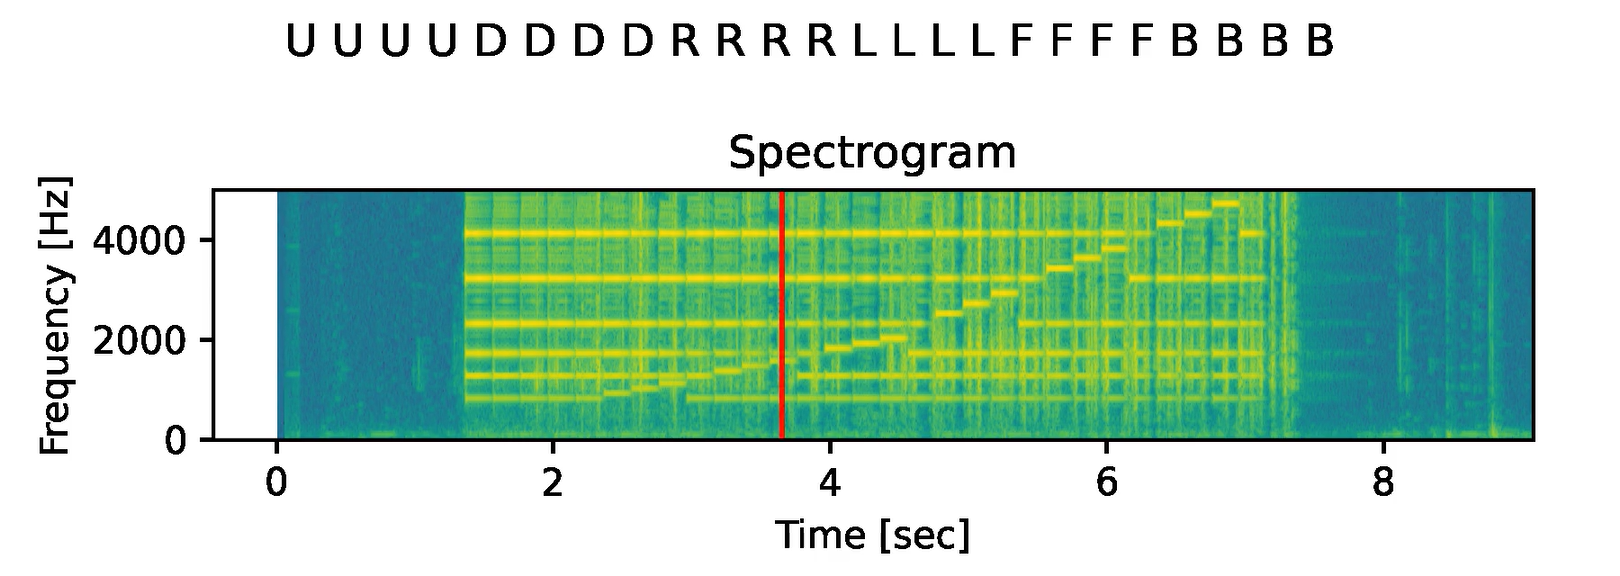
\includegraphics[width=0.8\linewidth]{Figures/5 Algorithm Design/transmitted-356-5tps.png}
\end{figure}

Notice how the horizontal bands representing the transmitted signal are
dimmer in the realistic audio than in the purely synthetic audio. This
reflects the loss of volume any tone experiences as it travels through
the air. Additionally, the transmitted signal is also partially
obscured by the additional audible noise of solving the speedcube.

\section{Decoding Realistic Audio}
\label{sec:decoding-realistic-noise}

The loss of signal strength alongside the added noise creates several
unique challenges that require more sophisticated analysis than that
presented in Section \ref{sec:decoding-synthetic-audio}. These
challenges include added variation in the strength of each peak
frequency (Section \ref{subsec:fine-tuning-threshold}), the detection
of conflicting centerpiece states (Section
\ref{subsec:filtering-similar-peak-frequencies}), and the erroneous
reading of background noise as centerpiece states (Section
\ref{subsec:ignoring-noise-when-extracting-move-sequences}).

\subsection{Fine-Tuning the Threshold}
\label{subsec:fine-tuning-threshold}

Because some audio frequencies are dampened more than others as they
travel through the air to the recording microphone, a static threshold
like the one used in Section \ref{subsec:extract-dominant-freqs} fails
to capture all the dominant frequencies that compose the audible
signal. For example, Figure \ref{fig:threshold-miss} shows how the 85\%
threshold from Section \ref{subsec:extract-dominant-freqs} misses five
of the six signal peaks in the realistic audio.

\begin{figure}[h]
    \centering
    \caption{An 85\% threshold applied to realistic audio}
    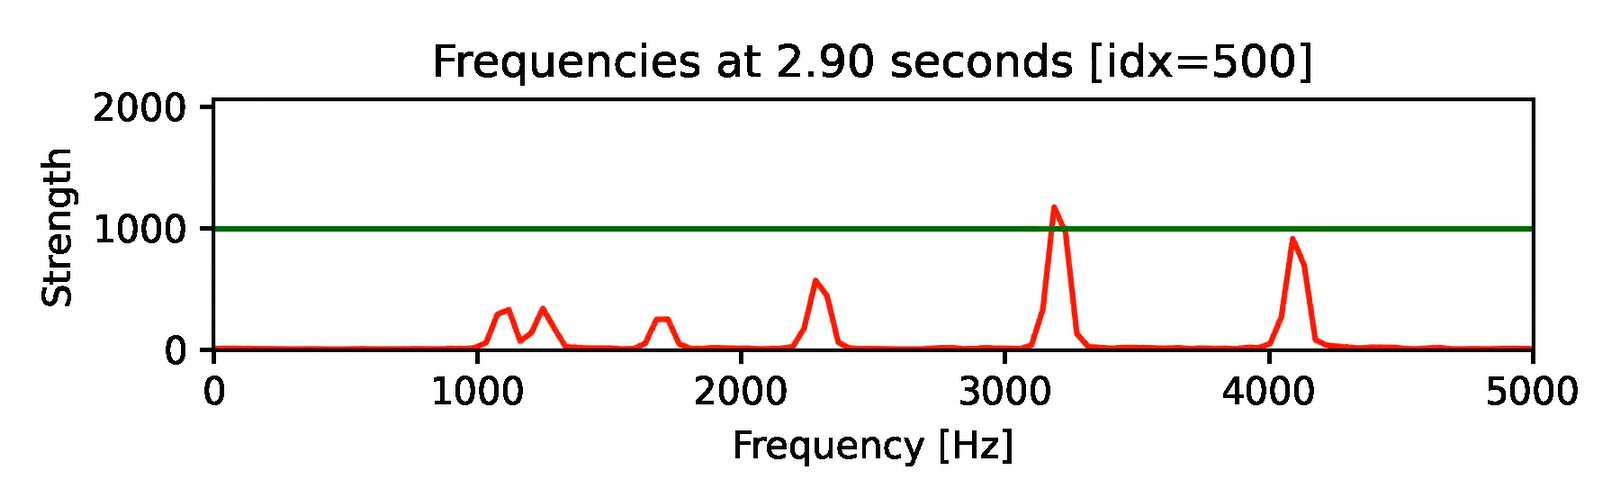
\includegraphics[width=0.8\linewidth]{Figures/5 Algorithm Design/threshold-miss.png}
    \label{fig:threshold-miss}
\end{figure}

Furthermore, the natural background noise can also cause false
positives during the moments between moves while the signal is weaker
as a result of changing from one state to the next. For example, Figure
\ref{fig:threshold-false-positives} shows a moment between face turns
when the audio signal is nearly non-existent, and the background noise
can falsely register as important peak frequencies for centerpiece
state detection. In this case, between 1000Hz and 2000Hz alone there
are six different points where the background noise reaches the 85\%
threshold compared to the three centerpieces who state gets transmitted
within that same band.

\begin{figure}[h]
    \centering
    \caption{Dominance of background noise between moves}
    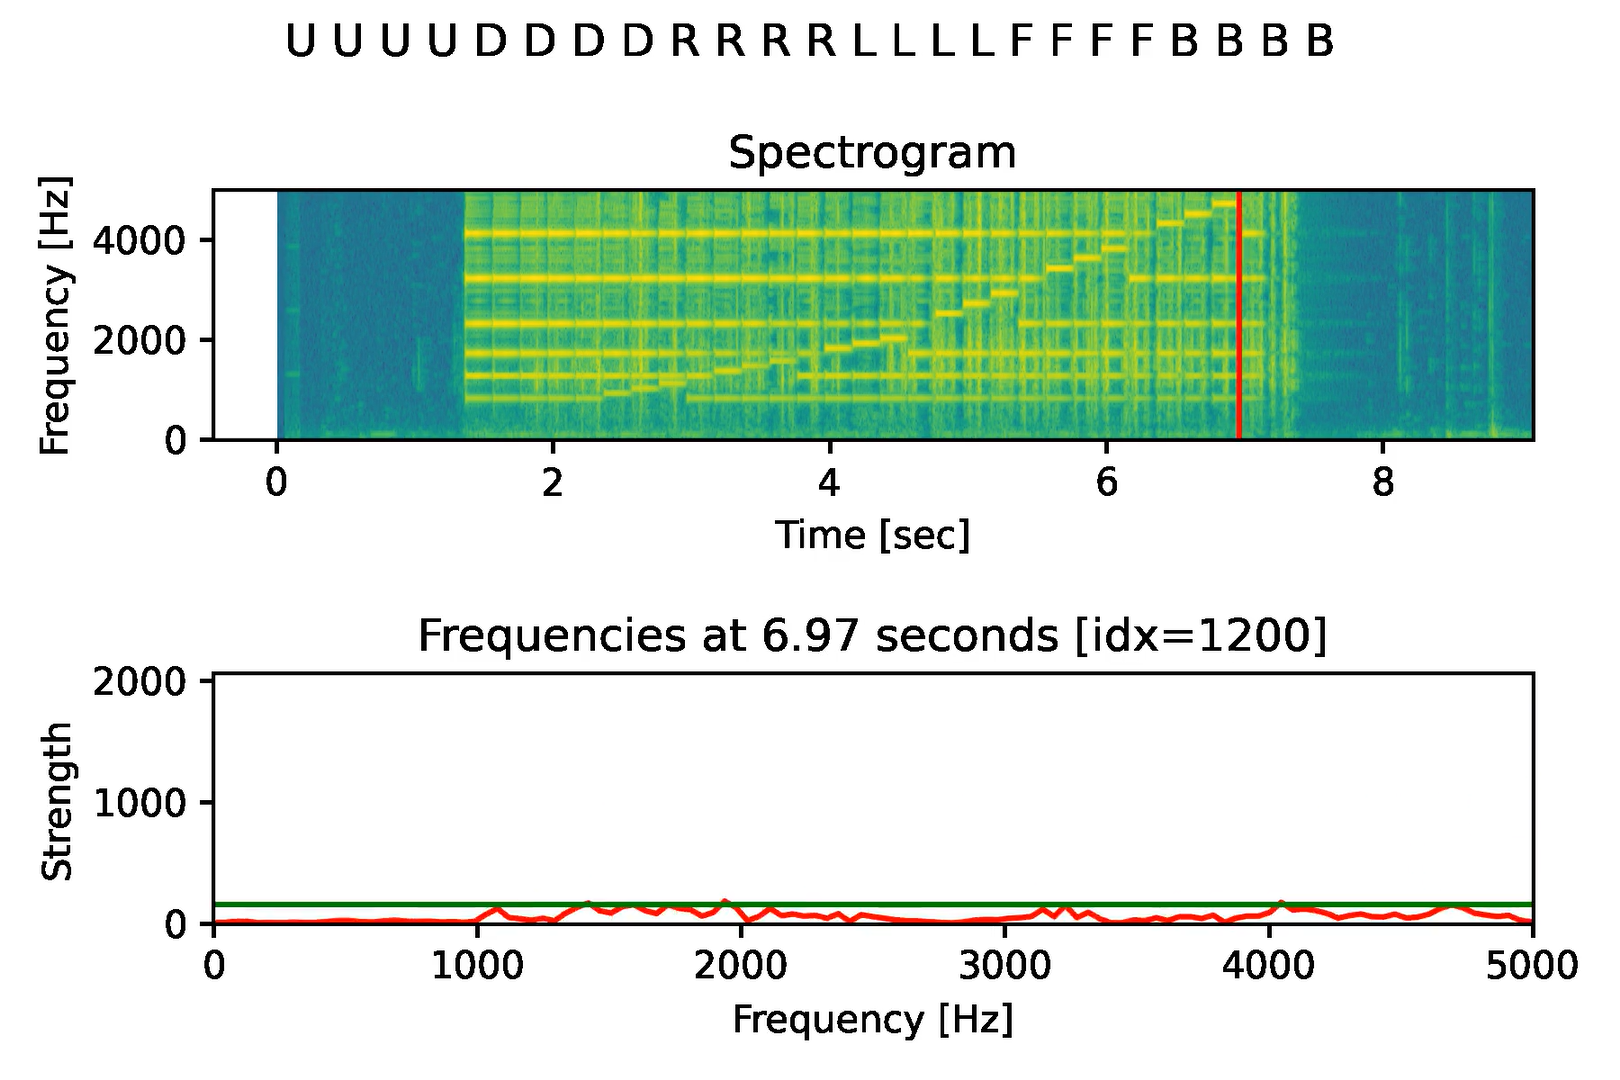
\includegraphics[width=0.8\linewidth]{Figures/5 Algorithm Design/threshold-false-positives.png}
    \label{fig:threshold-false-positives}
\end{figure}

\newpage

Resolving these issues starts by noticing that the power of each peak
frequency bearing the audio signal is generally much higher than the
power of all other component frequencies. As such, basing the threshold
at a power equal to one standard deviation of the power of the
component frequencies of a specific time step generally captures all
the peak frequencies while still excluding the underlying noise of the
cube/environment. Additionally, the use of a hard minimum value for the
threshold helps reduce the number of false positives during the gaps in
the signal between face turns.

These two changes are encoded in an updated version of the
\code{compute\_threshold} function first defined in Section
\ref{subsec:extract-dominant-freqs}. This new version contains two new
parameters: \code{stdv\_pct}, which can be used to adjust the threshold
to some multiple of the standard deviation for testing purposes, and
\code{min\_thresh} which is the "hard minimum value" discussed in the
previous paragraph.

\begin{figure}[h]
\caption{Updated version of threshold computation in Figure \ref{fig:code-compute-threshold}}
\label{fig:code-compute-threshold-v2}
\begin{lstlisting}[language=Python]
def compute_threshold(values: list, stdv_pct: float=1, min_thresh: int=50):
    return max(min_thresh, np.std(values) * stdv_pct)
\end{lstlisting}
\end{figure}

An example of the thresholds yielded by this new computation is shown
in Figure \ref{fig:threshold-refined}, where the green line
representing the threshold successfully captures all six peak
frequencies of the audio signal while simultaneously staying just out
of reach from the frequencies of the background noise.

\begin{figure}[h]
    \centering
    \caption{Fine-Tuned Threshold}
    \label{fig:threshold-refined}
    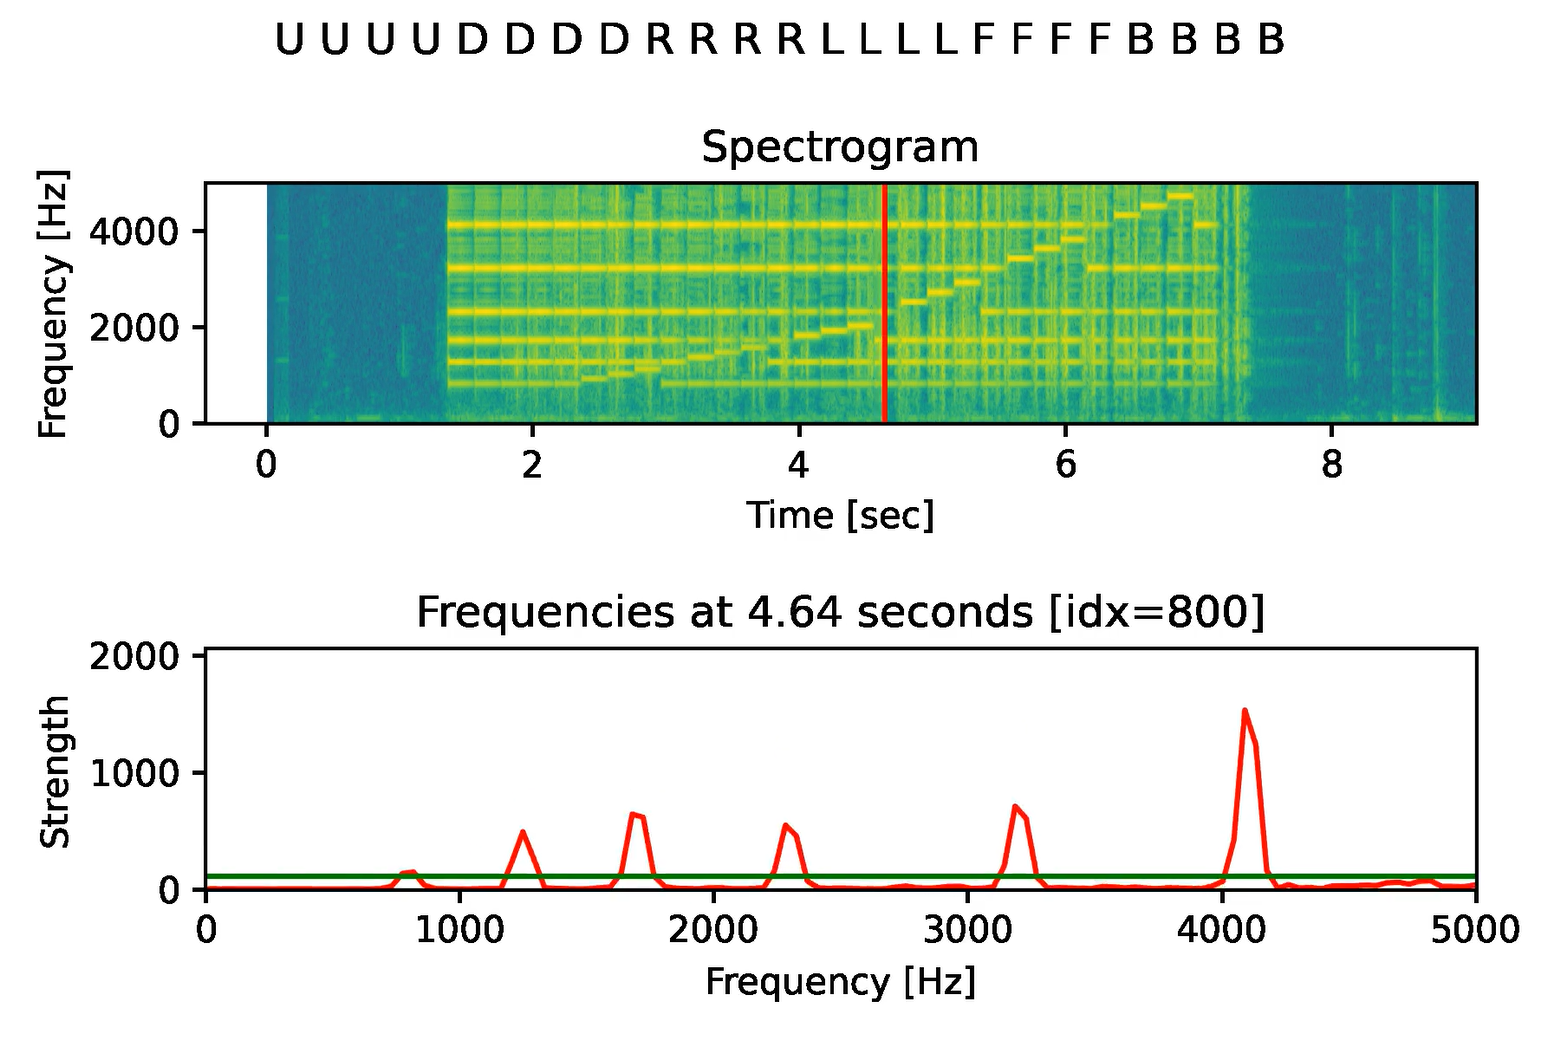
\includegraphics[width=0.8\linewidth]{Figures/5 Algorithm Design/threshold-refined.png}
\end{figure}

\newpage
\subsection{Filtering through Similar Peak Frequencies}
\label{subsec:filtering-similar-peak-frequencies}

While the new threshold calculation does properly capture all the peak
frequencies, it also captures more samples than just the six tips of
each peak. These extra samples can cause confusion when trying to
extract each centerpiece's state if they correspond to different states
for the same centerpiece. That said, as long as the power of each
frequency is also saved, then any disagreements about a specific
centerpiece's state can be resolved by accepting the one with the most
intense frequency as the actual state.

In code, this is achieved by adding a temporary dictionary to the
\code{get\_state\_by\_freqs} method defined in Section
\ref{subsec:translating-freqs-to-state} to track the strongest
frequency associated with each face. Then, while iterating through the
captured peak frequencies, only the strongest one for each face is used
to determine the active centerpiece state at that time step.

\begin{figure}[h]
\caption{Updated version of state extraction in Figure \ref{fig:code-extract-important-freqs}}
\label{fig:code-get-state-from-freqs-new}
\begin{lstlisting}[language=Python]
def get_state_from_freqs(important_freqs: list) -> dict:
    state = {}
    state_power = {"U": 0, "D": 0, "R": 0, "L": 0, "F": 0, "B": 0}  # New
    for freq in important_freqs:
        hz, power = freq.values()
        closest_state = _closest_state(hz)
        if power > state_power[closest_state["face"]]:              # New
            state[closest_state["face"]] = closest_state["rotation"]
            state_power[closest_state["face"]] = power              # New
    return state
\end{lstlisting}
\end{figure}

Using this new version of \code{get\_state\_by\_freqs} works just like
it did in Figure \ref{fig:code-get-state-from-freqs-demo}. Here the
extracted state is the one encoded by the frequencies depicted in
Figure \ref{fig:threshold-refined}.

\begin{figure}[h]
\caption{Example: Refined conversion of peak frequencies to states}
\label{fig:code-get-state-from-freqs-new-demo}
\begin{subfigure}{\textwidth}
\begin{lstlisting}[language=Python]
transmitted_wav_path = "transmitted-356-5tps.wav"
freq, time, spectrogram = compute_spectrogram(transmitted_wav_path)
important_freqs = extract_important_freqs(freq, time, spectrogram,
    t_idx=800) # 4.64 seconds

detected_state = get_state_from_freqs(important_freqs)
print(detected_state)
\end{lstlisting}
\end{subfigure}\\

\begin{subfigure}{\textwidth}
\begin{lstlisting}[language=Python, numbers=none]
>> {"U": 0, "D": 0, "R": 0, "L": 0, "F": 0, "B": 0}
\end{lstlisting}
\end{subfigure}
\end{figure}

\newpage
\subsection{Ignoring Noise when Extracting Move Sequences}
\label{subsec:ignoring-noise-when-extracting-move-sequences}

However, despite these noise filtering measures, the background noise
occasionally causes the detection of an incorrect centerpiece state.
Since the approach in Section \ref{subsec:extract-moves} registers an
applied face turn for \emph{any} detected change in a centerpiece's
state, \emph{any} mis-detection would incorrectly register a face turn
that never happened.

Fortunately, this issue can be mitigated by requiring that the state
change persists over several time steps instead of blindly accepting
any detected change in a centerpiece's state as a new face turn.

This is implemented by adding a sliding window to the
\code{detect\_moves} function first created in Section
\ref{subsec:extract-moves}. The window implementation starts with a new
\code{window\_size} function parameter to control the number of
consecutive time steps over which a state change has to persist before
it is recorded as a move applied to the cube. Within the function, two
new dictionaries are created to serve as a "staging area" for state
changes: one to stage the new state and the second to record the index
of the time step where the state first changed. As the function
iterates through each time step, it updates these staging dictionaries
each time a new state is detected. Then, it checks to see if the
current index of iteration is \code{window\_size} steps after the last
reported state change. If so, the current state is updated to the value
of the staged state, the change is recorded as a new move, and the
window counter gets reset. Otherwise, the iteration continues until a
new state is detected or the \code{window\_size} is reached. The full
code for this is shown in Figure \ref{fig:code-detect-moves-new}.


\begin{figure}[h]
\caption{Updated version of move detection in Figure \ref{fig:code-detect-moves}}
\label{fig:code-detect-moves-new}
\begin{lstlisting}[language=Python, mathescape]
def detect_moves(state_over_time, window_size=8):                 # Edit
    detected_moves = []
    current_state = {}
    new_state = {"U":-1, "D":-1, "R":-1, "L":-1, "F":-1, "B":-1}  # New
    new_state_idx = {"U":0, "D":0, "R":0, "L":0, "F":0, "B":0}    # New
    for idx, timed_state in enumerate(state_over_time):
        time, state = timed_state.values()
        for face, rotation in state.items():
            # Update new_state whenever the rotation changes      # Edit $\downarrow$
            if rotation != new_state[face]:
                new_state[face] = rotation
                new_state_idx[face] = idx
            # If the new state has persisted over window_size time steps,
            if idx - new_state_idx[face] == window_size:
                if not (face in current_state):
                    current_state[face] = new_state[face]
                # and it is a different rotation than the current state,
                elif new_state[face] != current_state[face]:
                    # then a face turn has been detected!
                    detected_moves.append(dict(
                        time=state_over_time[new_state_idx[face]]["time"],
                        move=_move_from(face, current_state[face], rotation)
                    ))
                    current_state[face] = rotation
                    new_state_idx[face] = 0
    return detected_moves
\end{lstlisting}
\end{figure}

And to validate that these changes work as expected, Figure
\ref{fig:code-detect-moves-new-demo} runs the realistic audio through
this new \code{detect\_moves} function and compares the returned move
sequence with the one originally transmitted in the audio.

\begin{figure}[h]
\caption{Example: Refined move sequence extraction}
\label{fig:code-detect-moves-new-demo}
\begin{subfigure}{\textwidth}
\begin{lstlisting}[language=Python]
state_over_time = get_state_over_time(freq, time, spectrogram)
detected_moves = detect_moves(state_over_time)

pretty_moves = " ".join([i["move"] for i in detected_moves])
print(pretty_moves)   
print(f"Matches demo_alg? {demo_alg == pretty_moves}")
\end{lstlisting}
\end{subfigure}\\

\begin{subfigure}{\textwidth}
\begin{lstlisting}[language=Python, numbers=none]
>> U U U U D D D D R R R R L L L L F F F F B B B B
>> Matches demo_alg? True
\end{lstlisting}
\end{subfigure}
\end{figure}

And once again, the detected move sequence perfectly matches the
transmitted signal despite both the reduced strength of the synthetic
audio after being recorded through the air and the presence of the
added noise of solving a speedcube, a result which further validates
this approach as a viable proof-of-concept for tracking the moves of a
Rubik's Cube using sound.

\subsection{Optimizing Algorithm Parameters}
\label{subsec:optimizing-params}

Significant testing went into determining the best default values for
each of the three new function parameters \code{stdv\_pct} (Section
\ref{subsec:fine-tuning-threshold}), \code{min\_thresh} (Section
\ref{subsec:fine-tuning-threshold}), and \code{window\_size} (Section
\ref{subsec:ignoring-noise-when-extracting-move-sequences}). While each
cube responded differently to various combinations of settings, this
testing discovered multiple combinations for each cube that would yield
a perfect extraction of the original move sequence. A detailed
exploration of this testing and its findings is discussed in Chapter
\ref{Chapter7}.

\section{Summary}

In summary, this chapter demonstrated a proof of concept for a sound
analysis algorithm that could detect the face turns of a speedcube
equipped with the proper transmitter (the details of which are explored
in Chapter \ref{Chapter6}). This proof of concept algorithm works by
computing the spectrogram of the transmitted audio, extracting the most
intense frequencies from each time step, converting those dominant
frequencies to centerpiece states at that time step, then iterating
through that list of states over time to detect changes caused by face
turns. Several noise mitigation measures were employed to help mitigate
the impact of loud cubes and other background tones. Ultimately, this
algorithm design successfully decoded both a purely synthetic audio
signal and a realistic audio signal created by re-recording the
synthetic audio while solving a speedcube.
